
% Default to the notebook output style

    


% Inherit from the specified cell style.




    
\documentclass[11pt]{article}

    
    
    \usepackage[T1]{fontenc}
    % Nicer default font (+ math font) than Computer Modern for most use cases
    \usepackage{mathpazo}

    % Basic figure setup, for now with no caption control since it's done
    % automatically by Pandoc (which extracts ![](path) syntax from Markdown).
    \usepackage{graphicx}
    % We will generate all images so they have a width \maxwidth. This means
    % that they will get their normal width if they fit onto the page, but
    % are scaled down if they would overflow the margins.
    \makeatletter
    \def\maxwidth{\ifdim\Gin@nat@width>\linewidth\linewidth
    \else\Gin@nat@width\fi}
    \makeatother
    \let\Oldincludegraphics\includegraphics
    % Set max figure width to be 80% of text width, for now hardcoded.
    \renewcommand{\includegraphics}[1]{\Oldincludegraphics[width=.8\maxwidth]{#1}}
    % Ensure that by default, figures have no caption (until we provide a
    % proper Figure object with a Caption API and a way to capture that
    % in the conversion process - todo).
    \usepackage{caption}
    \DeclareCaptionLabelFormat{nolabel}{}
    \captionsetup{labelformat=nolabel}

    \usepackage{adjustbox} % Used to constrain images to a maximum size 
    \usepackage{xcolor} % Allow colors to be defined
    \usepackage{enumerate} % Needed for markdown enumerations to work
    \usepackage{geometry} % Used to adjust the document margins
    \usepackage{amsmath} % Equations
    \usepackage{amssymb} % Equations
    \usepackage{textcomp} % defines textquotesingle
    % Hack from http://tex.stackexchange.com/a/47451/13684:
    \AtBeginDocument{%
        \def\PYZsq{\textquotesingle}% Upright quotes in Pygmentized code
    }
    \usepackage{upquote} % Upright quotes for verbatim code
    \usepackage{eurosym} % defines \euro
    \usepackage[mathletters]{ucs} % Extended unicode (utf-8) support
    \usepackage[utf8x]{inputenc} % Allow utf-8 characters in the tex document
    \usepackage{fancyvrb} % verbatim replacement that allows latex
    \usepackage{grffile} % extends the file name processing of package graphics 
                         % to support a larger range 
    % The hyperref package gives us a pdf with properly built
    % internal navigation ('pdf bookmarks' for the table of contents,
    % internal cross-reference links, web links for URLs, etc.)
    \usepackage{hyperref}
    \usepackage{longtable} % longtable support required by pandoc >1.10
    \usepackage{booktabs}  % table support for pandoc > 1.12.2
    \usepackage[inline]{enumitem} % IRkernel/repr support (it uses the enumerate* environment)
    \usepackage[normalem]{ulem} % ulem is needed to support strikethroughs (\sout)
                                % normalem makes italics be italics, not underlines
    

    
    
    % Colors for the hyperref package
    \definecolor{urlcolor}{rgb}{0,.145,.698}
    \definecolor{linkcolor}{rgb}{.71,0.21,0.01}
    \definecolor{citecolor}{rgb}{.12,.54,.11}

    % ANSI colors
    \definecolor{ansi-black}{HTML}{3E424D}
    \definecolor{ansi-black-intense}{HTML}{282C36}
    \definecolor{ansi-red}{HTML}{E75C58}
    \definecolor{ansi-red-intense}{HTML}{B22B31}
    \definecolor{ansi-green}{HTML}{00A250}
    \definecolor{ansi-green-intense}{HTML}{007427}
    \definecolor{ansi-yellow}{HTML}{DDB62B}
    \definecolor{ansi-yellow-intense}{HTML}{B27D12}
    \definecolor{ansi-blue}{HTML}{208FFB}
    \definecolor{ansi-blue-intense}{HTML}{0065CA}
    \definecolor{ansi-magenta}{HTML}{D160C4}
    \definecolor{ansi-magenta-intense}{HTML}{A03196}
    \definecolor{ansi-cyan}{HTML}{60C6C8}
    \definecolor{ansi-cyan-intense}{HTML}{258F8F}
    \definecolor{ansi-white}{HTML}{C5C1B4}
    \definecolor{ansi-white-intense}{HTML}{A1A6B2}

    % commands and environments needed by pandoc snippets
    % extracted from the output of `pandoc -s`
    \providecommand{\tightlist}{%
      \setlength{\itemsep}{0pt}\setlength{\parskip}{0pt}}
    \DefineVerbatimEnvironment{Highlighting}{Verbatim}{commandchars=\\\{\}}
    % Add ',fontsize=\small' for more characters per line
    \newenvironment{Shaded}{}{}
    \newcommand{\KeywordTok}[1]{\textcolor[rgb]{0.00,0.44,0.13}{\textbf{{#1}}}}
    \newcommand{\DataTypeTok}[1]{\textcolor[rgb]{0.56,0.13,0.00}{{#1}}}
    \newcommand{\DecValTok}[1]{\textcolor[rgb]{0.25,0.63,0.44}{{#1}}}
    \newcommand{\BaseNTok}[1]{\textcolor[rgb]{0.25,0.63,0.44}{{#1}}}
    \newcommand{\FloatTok}[1]{\textcolor[rgb]{0.25,0.63,0.44}{{#1}}}
    \newcommand{\CharTok}[1]{\textcolor[rgb]{0.25,0.44,0.63}{{#1}}}
    \newcommand{\StringTok}[1]{\textcolor[rgb]{0.25,0.44,0.63}{{#1}}}
    \newcommand{\CommentTok}[1]{\textcolor[rgb]{0.38,0.63,0.69}{\textit{{#1}}}}
    \newcommand{\OtherTok}[1]{\textcolor[rgb]{0.00,0.44,0.13}{{#1}}}
    \newcommand{\AlertTok}[1]{\textcolor[rgb]{1.00,0.00,0.00}{\textbf{{#1}}}}
    \newcommand{\FunctionTok}[1]{\textcolor[rgb]{0.02,0.16,0.49}{{#1}}}
    \newcommand{\RegionMarkerTok}[1]{{#1}}
    \newcommand{\ErrorTok}[1]{\textcolor[rgb]{1.00,0.00,0.00}{\textbf{{#1}}}}
    \newcommand{\NormalTok}[1]{{#1}}
    
    % Additional commands for more recent versions of Pandoc
    \newcommand{\ConstantTok}[1]{\textcolor[rgb]{0.53,0.00,0.00}{{#1}}}
    \newcommand{\SpecialCharTok}[1]{\textcolor[rgb]{0.25,0.44,0.63}{{#1}}}
    \newcommand{\VerbatimStringTok}[1]{\textcolor[rgb]{0.25,0.44,0.63}{{#1}}}
    \newcommand{\SpecialStringTok}[1]{\textcolor[rgb]{0.73,0.40,0.53}{{#1}}}
    \newcommand{\ImportTok}[1]{{#1}}
    \newcommand{\DocumentationTok}[1]{\textcolor[rgb]{0.73,0.13,0.13}{\textit{{#1}}}}
    \newcommand{\AnnotationTok}[1]{\textcolor[rgb]{0.38,0.63,0.69}{\textbf{\textit{{#1}}}}}
    \newcommand{\CommentVarTok}[1]{\textcolor[rgb]{0.38,0.63,0.69}{\textbf{\textit{{#1}}}}}
    \newcommand{\VariableTok}[1]{\textcolor[rgb]{0.10,0.09,0.49}{{#1}}}
    \newcommand{\ControlFlowTok}[1]{\textcolor[rgb]{0.00,0.44,0.13}{\textbf{{#1}}}}
    \newcommand{\OperatorTok}[1]{\textcolor[rgb]{0.40,0.40,0.40}{{#1}}}
    \newcommand{\BuiltInTok}[1]{{#1}}
    \newcommand{\ExtensionTok}[1]{{#1}}
    \newcommand{\PreprocessorTok}[1]{\textcolor[rgb]{0.74,0.48,0.00}{{#1}}}
    \newcommand{\AttributeTok}[1]{\textcolor[rgb]{0.49,0.56,0.16}{{#1}}}
    \newcommand{\InformationTok}[1]{\textcolor[rgb]{0.38,0.63,0.69}{\textbf{\textit{{#1}}}}}
    \newcommand{\WarningTok}[1]{\textcolor[rgb]{0.38,0.63,0.69}{\textbf{\textit{{#1}}}}}
    
    
    % Define a nice break command that doesn't care if a line doesn't already
    % exist.
    \def\br{\hspace*{\fill} \\* }
    % Math Jax compatability definitions
    \def\gt{>}
    \def\lt{<}
    % Document parameters
    \title{writeup\_report}
    
    
    

    % Pygments definitions
    
\makeatletter
\def\PY@reset{\let\PY@it=\relax \let\PY@bf=\relax%
    \let\PY@ul=\relax \let\PY@tc=\relax%
    \let\PY@bc=\relax \let\PY@ff=\relax}
\def\PY@tok#1{\csname PY@tok@#1\endcsname}
\def\PY@toks#1+{\ifx\relax#1\empty\else%
    \PY@tok{#1}\expandafter\PY@toks\fi}
\def\PY@do#1{\PY@bc{\PY@tc{\PY@ul{%
    \PY@it{\PY@bf{\PY@ff{#1}}}}}}}
\def\PY#1#2{\PY@reset\PY@toks#1+\relax+\PY@do{#2}}

\expandafter\def\csname PY@tok@gs\endcsname{\let\PY@bf=\textbf}
\expandafter\def\csname PY@tok@nv\endcsname{\def\PY@tc##1{\textcolor[rgb]{0.10,0.09,0.49}{##1}}}
\expandafter\def\csname PY@tok@sr\endcsname{\def\PY@tc##1{\textcolor[rgb]{0.73,0.40,0.53}{##1}}}
\expandafter\def\csname PY@tok@kc\endcsname{\let\PY@bf=\textbf\def\PY@tc##1{\textcolor[rgb]{0.00,0.50,0.00}{##1}}}
\expandafter\def\csname PY@tok@gr\endcsname{\def\PY@tc##1{\textcolor[rgb]{1.00,0.00,0.00}{##1}}}
\expandafter\def\csname PY@tok@ge\endcsname{\let\PY@it=\textit}
\expandafter\def\csname PY@tok@sx\endcsname{\def\PY@tc##1{\textcolor[rgb]{0.00,0.50,0.00}{##1}}}
\expandafter\def\csname PY@tok@nd\endcsname{\def\PY@tc##1{\textcolor[rgb]{0.67,0.13,1.00}{##1}}}
\expandafter\def\csname PY@tok@si\endcsname{\let\PY@bf=\textbf\def\PY@tc##1{\textcolor[rgb]{0.73,0.40,0.53}{##1}}}
\expandafter\def\csname PY@tok@ch\endcsname{\let\PY@it=\textit\def\PY@tc##1{\textcolor[rgb]{0.25,0.50,0.50}{##1}}}
\expandafter\def\csname PY@tok@ni\endcsname{\let\PY@bf=\textbf\def\PY@tc##1{\textcolor[rgb]{0.60,0.60,0.60}{##1}}}
\expandafter\def\csname PY@tok@nn\endcsname{\let\PY@bf=\textbf\def\PY@tc##1{\textcolor[rgb]{0.00,0.00,1.00}{##1}}}
\expandafter\def\csname PY@tok@ow\endcsname{\let\PY@bf=\textbf\def\PY@tc##1{\textcolor[rgb]{0.67,0.13,1.00}{##1}}}
\expandafter\def\csname PY@tok@kr\endcsname{\let\PY@bf=\textbf\def\PY@tc##1{\textcolor[rgb]{0.00,0.50,0.00}{##1}}}
\expandafter\def\csname PY@tok@gp\endcsname{\let\PY@bf=\textbf\def\PY@tc##1{\textcolor[rgb]{0.00,0.00,0.50}{##1}}}
\expandafter\def\csname PY@tok@cm\endcsname{\let\PY@it=\textit\def\PY@tc##1{\textcolor[rgb]{0.25,0.50,0.50}{##1}}}
\expandafter\def\csname PY@tok@s\endcsname{\def\PY@tc##1{\textcolor[rgb]{0.73,0.13,0.13}{##1}}}
\expandafter\def\csname PY@tok@bp\endcsname{\def\PY@tc##1{\textcolor[rgb]{0.00,0.50,0.00}{##1}}}
\expandafter\def\csname PY@tok@sb\endcsname{\def\PY@tc##1{\textcolor[rgb]{0.73,0.13,0.13}{##1}}}
\expandafter\def\csname PY@tok@kn\endcsname{\let\PY@bf=\textbf\def\PY@tc##1{\textcolor[rgb]{0.00,0.50,0.00}{##1}}}
\expandafter\def\csname PY@tok@no\endcsname{\def\PY@tc##1{\textcolor[rgb]{0.53,0.00,0.00}{##1}}}
\expandafter\def\csname PY@tok@c\endcsname{\let\PY@it=\textit\def\PY@tc##1{\textcolor[rgb]{0.25,0.50,0.50}{##1}}}
\expandafter\def\csname PY@tok@err\endcsname{\def\PY@bc##1{\setlength{\fboxsep}{0pt}\fcolorbox[rgb]{1.00,0.00,0.00}{1,1,1}{\strut ##1}}}
\expandafter\def\csname PY@tok@mo\endcsname{\def\PY@tc##1{\textcolor[rgb]{0.40,0.40,0.40}{##1}}}
\expandafter\def\csname PY@tok@w\endcsname{\def\PY@tc##1{\textcolor[rgb]{0.73,0.73,0.73}{##1}}}
\expandafter\def\csname PY@tok@vg\endcsname{\def\PY@tc##1{\textcolor[rgb]{0.10,0.09,0.49}{##1}}}
\expandafter\def\csname PY@tok@nc\endcsname{\let\PY@bf=\textbf\def\PY@tc##1{\textcolor[rgb]{0.00,0.00,1.00}{##1}}}
\expandafter\def\csname PY@tok@mh\endcsname{\def\PY@tc##1{\textcolor[rgb]{0.40,0.40,0.40}{##1}}}
\expandafter\def\csname PY@tok@nt\endcsname{\let\PY@bf=\textbf\def\PY@tc##1{\textcolor[rgb]{0.00,0.50,0.00}{##1}}}
\expandafter\def\csname PY@tok@nf\endcsname{\def\PY@tc##1{\textcolor[rgb]{0.00,0.00,1.00}{##1}}}
\expandafter\def\csname PY@tok@vm\endcsname{\def\PY@tc##1{\textcolor[rgb]{0.10,0.09,0.49}{##1}}}
\expandafter\def\csname PY@tok@m\endcsname{\def\PY@tc##1{\textcolor[rgb]{0.40,0.40,0.40}{##1}}}
\expandafter\def\csname PY@tok@se\endcsname{\let\PY@bf=\textbf\def\PY@tc##1{\textcolor[rgb]{0.73,0.40,0.13}{##1}}}
\expandafter\def\csname PY@tok@cs\endcsname{\let\PY@it=\textit\def\PY@tc##1{\textcolor[rgb]{0.25,0.50,0.50}{##1}}}
\expandafter\def\csname PY@tok@o\endcsname{\def\PY@tc##1{\textcolor[rgb]{0.40,0.40,0.40}{##1}}}
\expandafter\def\csname PY@tok@mi\endcsname{\def\PY@tc##1{\textcolor[rgb]{0.40,0.40,0.40}{##1}}}
\expandafter\def\csname PY@tok@sh\endcsname{\def\PY@tc##1{\textcolor[rgb]{0.73,0.13,0.13}{##1}}}
\expandafter\def\csname PY@tok@sd\endcsname{\let\PY@it=\textit\def\PY@tc##1{\textcolor[rgb]{0.73,0.13,0.13}{##1}}}
\expandafter\def\csname PY@tok@ne\endcsname{\let\PY@bf=\textbf\def\PY@tc##1{\textcolor[rgb]{0.82,0.25,0.23}{##1}}}
\expandafter\def\csname PY@tok@c1\endcsname{\let\PY@it=\textit\def\PY@tc##1{\textcolor[rgb]{0.25,0.50,0.50}{##1}}}
\expandafter\def\csname PY@tok@kt\endcsname{\def\PY@tc##1{\textcolor[rgb]{0.69,0.00,0.25}{##1}}}
\expandafter\def\csname PY@tok@mf\endcsname{\def\PY@tc##1{\textcolor[rgb]{0.40,0.40,0.40}{##1}}}
\expandafter\def\csname PY@tok@na\endcsname{\def\PY@tc##1{\textcolor[rgb]{0.49,0.56,0.16}{##1}}}
\expandafter\def\csname PY@tok@vc\endcsname{\def\PY@tc##1{\textcolor[rgb]{0.10,0.09,0.49}{##1}}}
\expandafter\def\csname PY@tok@mb\endcsname{\def\PY@tc##1{\textcolor[rgb]{0.40,0.40,0.40}{##1}}}
\expandafter\def\csname PY@tok@dl\endcsname{\def\PY@tc##1{\textcolor[rgb]{0.73,0.13,0.13}{##1}}}
\expandafter\def\csname PY@tok@gi\endcsname{\def\PY@tc##1{\textcolor[rgb]{0.00,0.63,0.00}{##1}}}
\expandafter\def\csname PY@tok@vi\endcsname{\def\PY@tc##1{\textcolor[rgb]{0.10,0.09,0.49}{##1}}}
\expandafter\def\csname PY@tok@gu\endcsname{\let\PY@bf=\textbf\def\PY@tc##1{\textcolor[rgb]{0.50,0.00,0.50}{##1}}}
\expandafter\def\csname PY@tok@sa\endcsname{\def\PY@tc##1{\textcolor[rgb]{0.73,0.13,0.13}{##1}}}
\expandafter\def\csname PY@tok@kp\endcsname{\def\PY@tc##1{\textcolor[rgb]{0.00,0.50,0.00}{##1}}}
\expandafter\def\csname PY@tok@nb\endcsname{\def\PY@tc##1{\textcolor[rgb]{0.00,0.50,0.00}{##1}}}
\expandafter\def\csname PY@tok@kd\endcsname{\let\PY@bf=\textbf\def\PY@tc##1{\textcolor[rgb]{0.00,0.50,0.00}{##1}}}
\expandafter\def\csname PY@tok@s2\endcsname{\def\PY@tc##1{\textcolor[rgb]{0.73,0.13,0.13}{##1}}}
\expandafter\def\csname PY@tok@ss\endcsname{\def\PY@tc##1{\textcolor[rgb]{0.10,0.09,0.49}{##1}}}
\expandafter\def\csname PY@tok@go\endcsname{\def\PY@tc##1{\textcolor[rgb]{0.53,0.53,0.53}{##1}}}
\expandafter\def\csname PY@tok@cpf\endcsname{\let\PY@it=\textit\def\PY@tc##1{\textcolor[rgb]{0.25,0.50,0.50}{##1}}}
\expandafter\def\csname PY@tok@fm\endcsname{\def\PY@tc##1{\textcolor[rgb]{0.00,0.00,1.00}{##1}}}
\expandafter\def\csname PY@tok@gd\endcsname{\def\PY@tc##1{\textcolor[rgb]{0.63,0.00,0.00}{##1}}}
\expandafter\def\csname PY@tok@s1\endcsname{\def\PY@tc##1{\textcolor[rgb]{0.73,0.13,0.13}{##1}}}
\expandafter\def\csname PY@tok@nl\endcsname{\def\PY@tc##1{\textcolor[rgb]{0.63,0.63,0.00}{##1}}}
\expandafter\def\csname PY@tok@il\endcsname{\def\PY@tc##1{\textcolor[rgb]{0.40,0.40,0.40}{##1}}}
\expandafter\def\csname PY@tok@gh\endcsname{\let\PY@bf=\textbf\def\PY@tc##1{\textcolor[rgb]{0.00,0.00,0.50}{##1}}}
\expandafter\def\csname PY@tok@gt\endcsname{\def\PY@tc##1{\textcolor[rgb]{0.00,0.27,0.87}{##1}}}
\expandafter\def\csname PY@tok@cp\endcsname{\def\PY@tc##1{\textcolor[rgb]{0.74,0.48,0.00}{##1}}}
\expandafter\def\csname PY@tok@k\endcsname{\let\PY@bf=\textbf\def\PY@tc##1{\textcolor[rgb]{0.00,0.50,0.00}{##1}}}
\expandafter\def\csname PY@tok@sc\endcsname{\def\PY@tc##1{\textcolor[rgb]{0.73,0.13,0.13}{##1}}}

\def\PYZbs{\char`\\}
\def\PYZus{\char`\_}
\def\PYZob{\char`\{}
\def\PYZcb{\char`\}}
\def\PYZca{\char`\^}
\def\PYZam{\char`\&}
\def\PYZlt{\char`\<}
\def\PYZgt{\char`\>}
\def\PYZsh{\char`\#}
\def\PYZpc{\char`\%}
\def\PYZdl{\char`\$}
\def\PYZhy{\char`\-}
\def\PYZsq{\char`\'}
\def\PYZdq{\char`\"}
\def\PYZti{\char`\~}
% for compatibility with earlier versions
\def\PYZat{@}
\def\PYZlb{[}
\def\PYZrb{]}
\makeatother


    % Exact colors from NB
    \definecolor{incolor}{rgb}{0.0, 0.0, 0.5}
    \definecolor{outcolor}{rgb}{0.545, 0.0, 0.0}



    
    % Prevent overflowing lines due to hard-to-break entities
    \sloppy 
    % Setup hyperref package
    \hypersetup{
      breaklinks=true,  % so long urls are correctly broken across lines
      colorlinks=true,
      urlcolor=urlcolor,
      linkcolor=linkcolor,
      citecolor=citecolor,
      }
    % Slightly bigger margins than the latex defaults
    
    \geometry{verbose,tmargin=1in,bmargin=1in,lmargin=1in,rmargin=1in}
    
    

    \begin{document}
    
    
    \maketitle
    
    

    
    \hypertarget{finding-lane-lines-on-the-road-by-mohamed-eltohamy}{%
\subsection{\texorpdfstring{\# Finding Lane Lines on the Road By
\emph{Mohamed
Eltohamy}}{\# Finding Lane Lines on the Road By Mohamed Eltohamy}}\label{finding-lane-lines-on-the-road-by-mohamed-eltohamy}}

    \hypertarget{the-goal-of-this-project-is-to-identify-lane-lines-on-the-road-and-draw-them-on-the-test-images-and-videos.-ill-be-explaining-how-i-managed-to-do-that-using-the-pipeline-i-created-that-employed-techniques-i-learned-in-this-course-and-others-that-i-learned-through-the-course-of-this-project.}{%
\paragraph{The goal of this project is to identify lane lines on the
road and draw them on the test images and videos. I'll be explaining how
I managed to do that using the pipeline I created that employed
techniques I learned in this course and others that I learned through
the course of this
project.}\label{the-goal-of-this-project-is-to-identify-lane-lines-on-the-road-and-draw-them-on-the-test-images-and-videos.-ill-be-explaining-how-i-managed-to-do-that-using-the-pipeline-i-created-that-employed-techniques-i-learned-in-this-course-and-others-that-i-learned-through-the-course-of-this-project.}}

    \hypertarget{reflection}{%
\subsection{\# Reflection}\label{reflection}}

\hypertarget{the-pipeline}{%
\subsection{1. The Pipeline}\label{the-pipeline}}

\hypertarget{the-pipeline-consists-of}{%
\paragraph{The Pipeline consists of:}\label{the-pipeline-consists-of}}

\begin{itemize}
\tightlist
\item
  Section \ref{22color20selection22}
\item
  Section \ref{grayscaling20and20smoothing20the20image}
\item
  Section \ref{canny20edge20detection}
\item
  Section \ref{region20of20interest}
\item
  Section \ref{hough20transform}
\item
  Section \ref{extrapolating20lane20lines}
\end{itemize}

Throughout the course of the project I will be showing the
transformations on this set of test images:

\begin{figure}
\centering
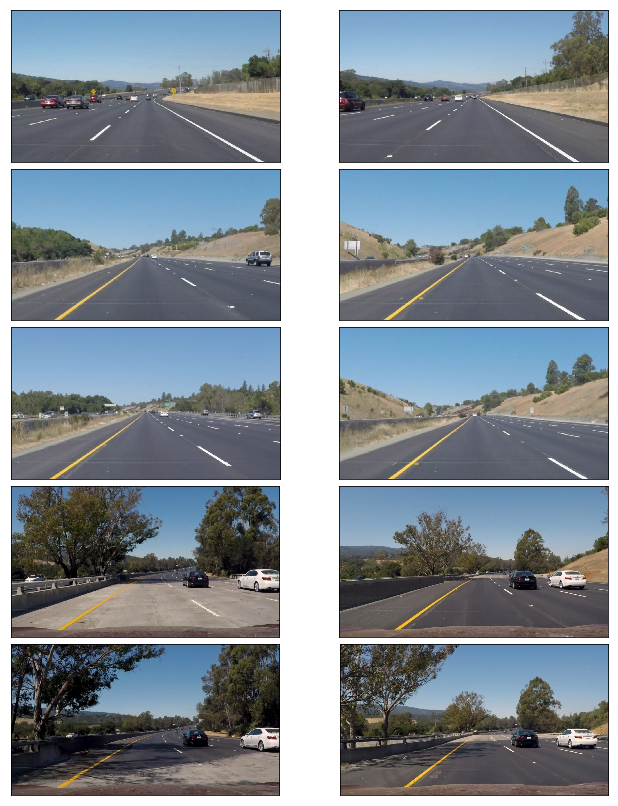
\includegraphics{test_images_output/all_test_images.png}
\caption{All Test Images}
\end{figure}

I went ahead and borrowed \emph{four} images form the challenge video to
include it in the test images as seen in the last four images. I did
that cause I wanted to test on images that have more noise like shade
and different lighting.

    \hypertarget{color-selection}{%
\subsection{\#\# Color Selection}\label{color-selection}}

Here I applied multiple strategies to get the \textbf{white} and
\textbf{yellow} lane lines from the test images.

\hypertarget{rgb-filtering}{%
\subsubsection{RGB filtering}\label{rgb-filtering}}

I first tried to use \textbf{RGB} filtering by applying a \emph{white}
and \emph{yellow} masks on the image and here were the results:

\begin{figure}
\centering
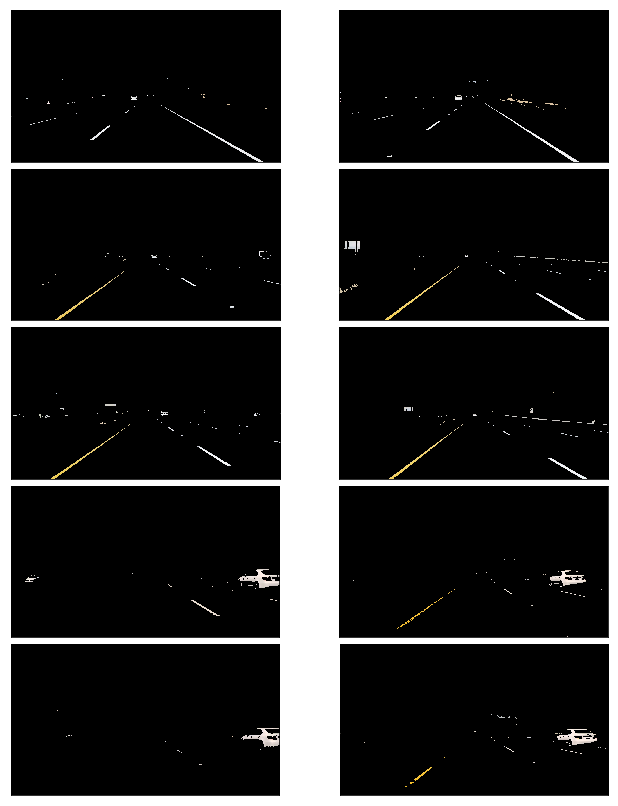
\includegraphics{test_images_output/rgb_filtered_test_images.png}
\caption{RGB filtering}
\end{figure}

While this gives good results for some images it lacks to detect the
lines for others like the images at the bottom which are mainly in the
shade.

So instead of using the default \textbf{RGB} color space which didn't
fit my data I went and explored two other color spaces:

\begin{itemize}
\tightlist
\item
  \textbf{HSV} which stands for Hue, Saturation, and Value
\item
  \textbf{HSL} which stands for Hue, Saturation, and Lightness
\end{itemize}

I used OpenCV's \texttt{cv2.cvtColor()} method to convert to each of the
color spaces.

Here are the results for the \textbf{HSV} color space:
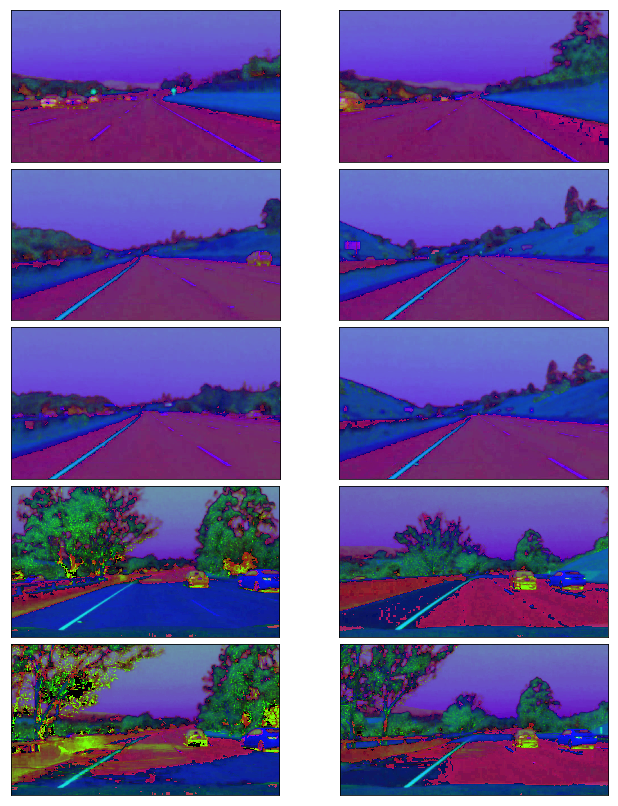
\includegraphics{test_images_output/hsv_test_images.png}

The \textbf{HSV} images clearly highlights the lane lines that are in
the shaded area in the bottom 4 images something that our \textbf{RGB}
filters lacked to accomplish;However, as you can see we lost all the
lane lines in the top two images, the white lines aren't really visible
especially the white dotted lines.

Then I checkout the \textbf{HSL} images:

\begin{figure}
\centering
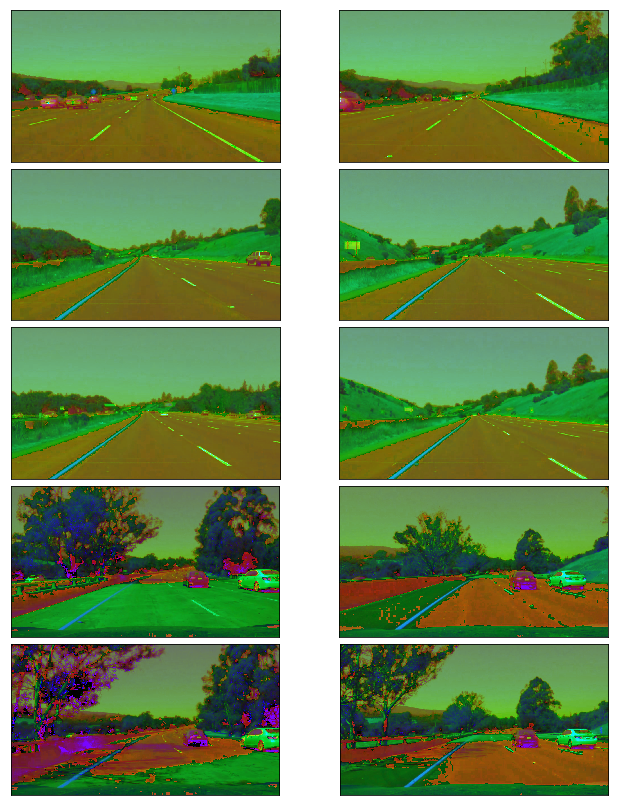
\includegraphics{test_images_output/hsl_test_images.png}
\caption{HSL test images}
\end{figure}

All lane lines are visible even the ones in the shade which is what was
missing from the \textbf{RGB} images after filtering, so I ended up
choosing the \textbf{HSL} images as the color space encompassed the best
of both worlds.

Then I used a white/yellow mask to isolate the white and yellow colors
in the image as show below:

\begin{figure}
\centering
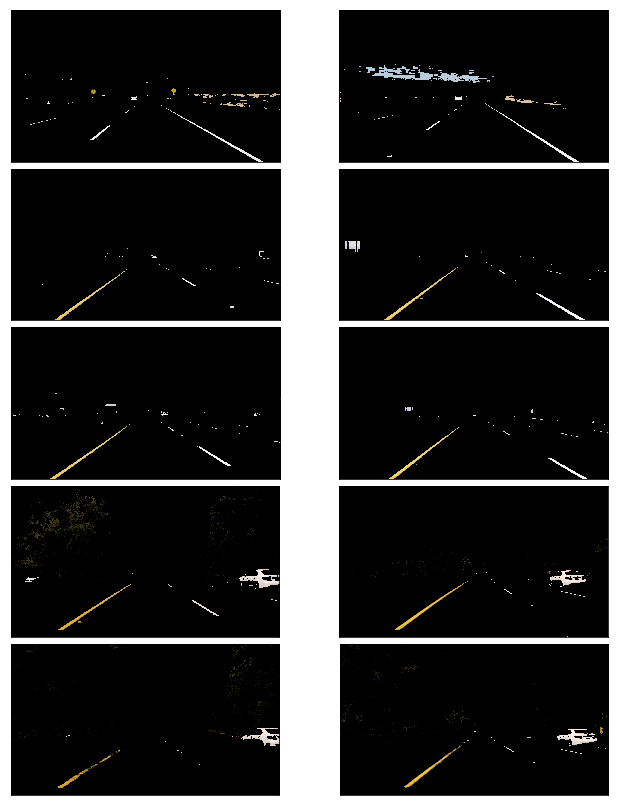
\includegraphics{test_images_output/white_yellow_filtered_hsl_images.png}
\caption{white/yellow filtered test images}
\end{figure}

\hypertarget{gray-scaling-and-smooting}{%
\subsection{\#\# Gray Scaling and
Smooting}\label{gray-scaling-and-smooting}}

After that I applies \textbf{grayscaling} on the images as shown here:

\begin{figure}
\centering
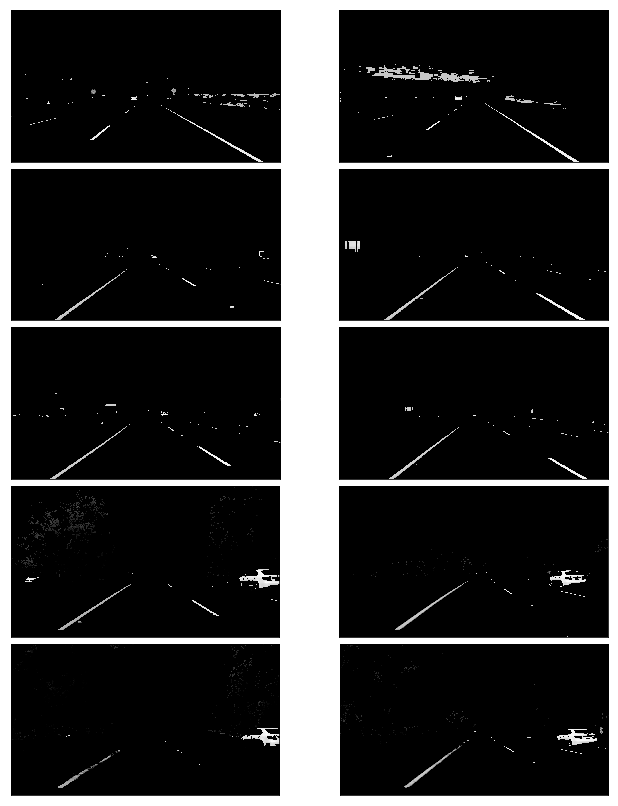
\includegraphics{test_images_output/grayscaled_test_images.png}
\caption{grayscaled test images}
\end{figure}

Then I applied smoothing the grayscaled image using \textbf{Gaussian
Blur} before I applied \textbf{Canny edge detection}, I found that a
filter size of 11 does a nice job on the sample images. Though
\textbf{Canny Edge Detection} applies smoothing internally, we can't
change the filter size so prior smoothing is recommended as a good
practice.

Here are the results of the images after smoothing:

\begin{figure}
\centering
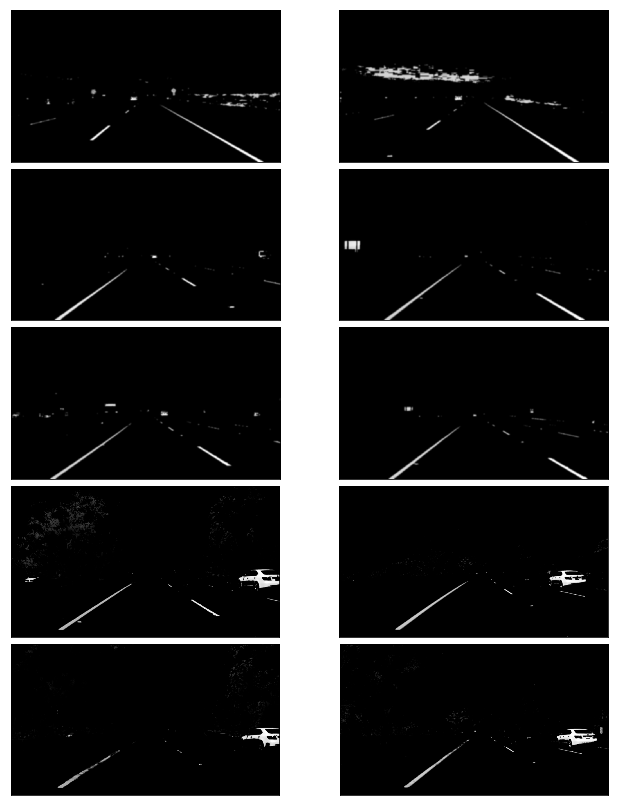
\includegraphics{test_images_output/smooth_test_images.png}
\caption{smoothed test images}
\end{figure}

\hypertarget{canny-edge-detection}{%
\subsection{\#\# Canny Edge Detection}\label{canny-edge-detection}}

Then I applied \textbf{Canny edge detection} with the thresholds of
\emph{50} to \emph{150} which is \emph{1:3 ratio} as recommended by
\textbf{Canny}, and here are the results:

\begin{figure}
\centering
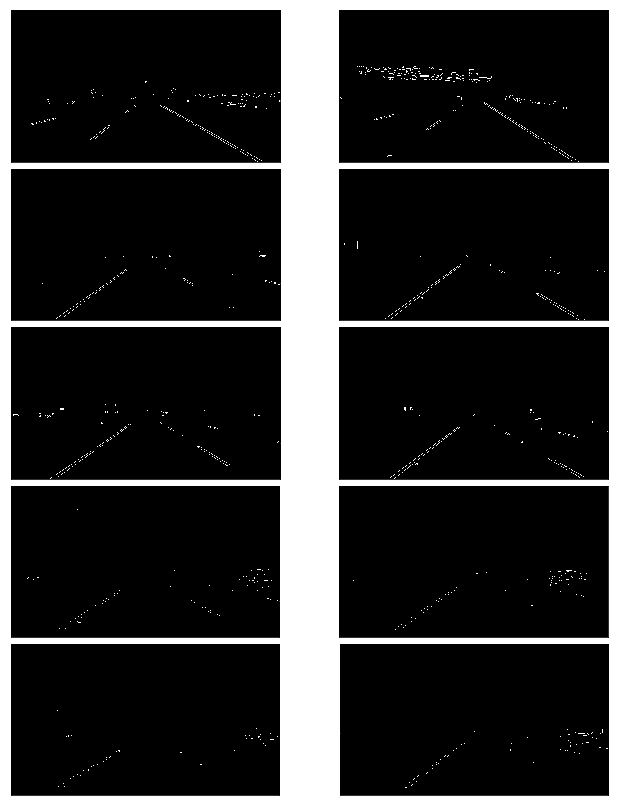
\includegraphics{test_images_output/canny_test_images.png}
\caption{Canny test images}
\end{figure}

\hypertarget{region-of-interest}{%
\subsection{\#\# Region of interest}\label{region-of-interest}}

After \textbf{selecting the colors, gray scaling, smoothing, and getting
the image's Canny edges} I removed all the unimportant parts of the
image like other lane lines, trees, sky, etc. to focus on the road
ahead. I did this by applying a mask to only include pixels within a
region of interest, and here is the results after applying it on the
\textbf{Canny} images:

\begin{figure}
\centering
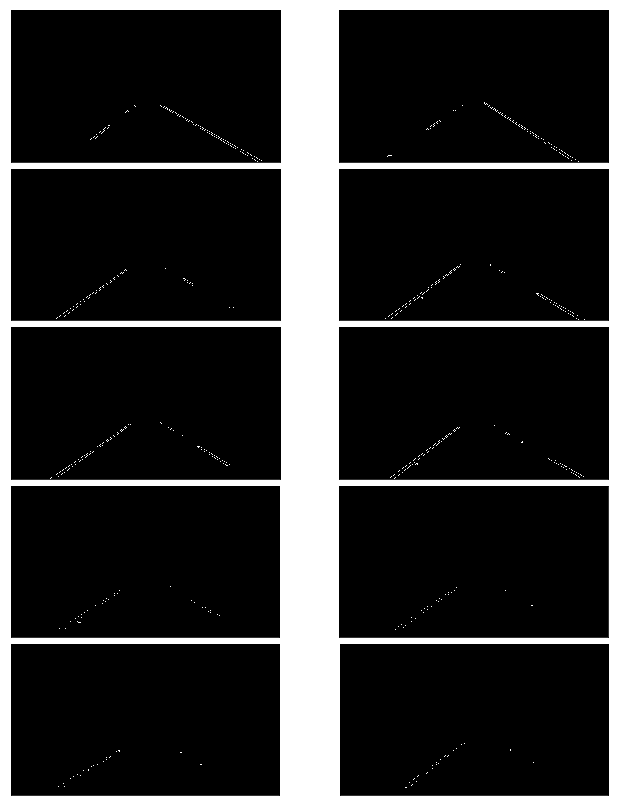
\includegraphics{test_images_output/regionofinterest_test_images.png}
\caption{Region of interest test images}
\end{figure}

As you can see I got a good \emph{outlines} of the lane lines, the
region of interest is as follows:

\begin{itemize}
\tightlist
\item
  Bottom is set to the image bottom
\item
  Top is set to \emph{60\%} of the image hight(just below the image
  center) which I think is a good estimate for the horizon
\item
  Its width spans the image with a little padding 5\% to eachside and
  narrows towards the top of the image with a width of 10\%
\end{itemize}

This gives a good representation of a road with its lane lines narrowing
toward the horizon.

\hypertarget{hough-transform}{%
\subsection{\#\# Hough Transform}\label{hough-transform}}

I then proceeded to apply the \textbf{Hough transform} which resulted in
the lines below:

\begin{figure}
\centering
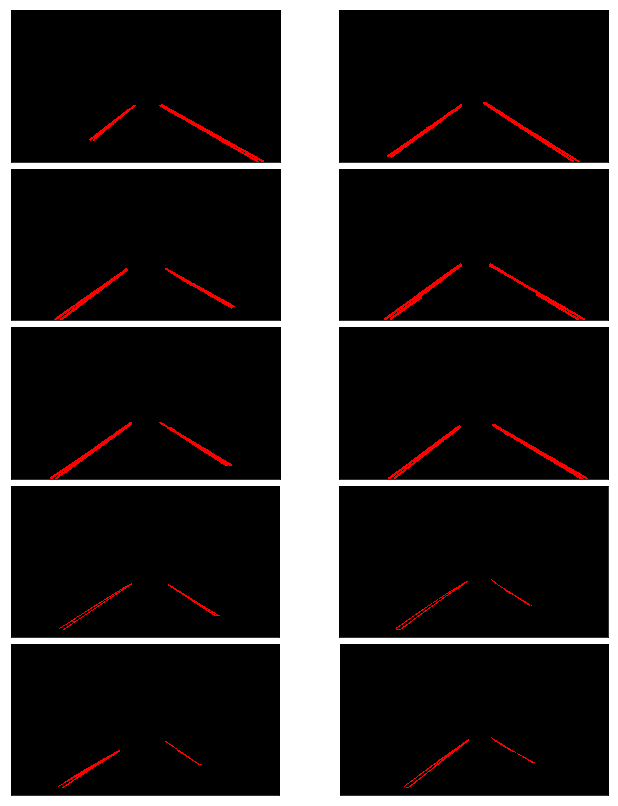
\includegraphics{test_images_output/hough_lines_test_images.png}
\caption{Hough lines test images}
\end{figure}

This result is pretty good for it show clear lines where the lane lines
are, here are the lines drawn on top of the real images:

\begin{figure}
\centering
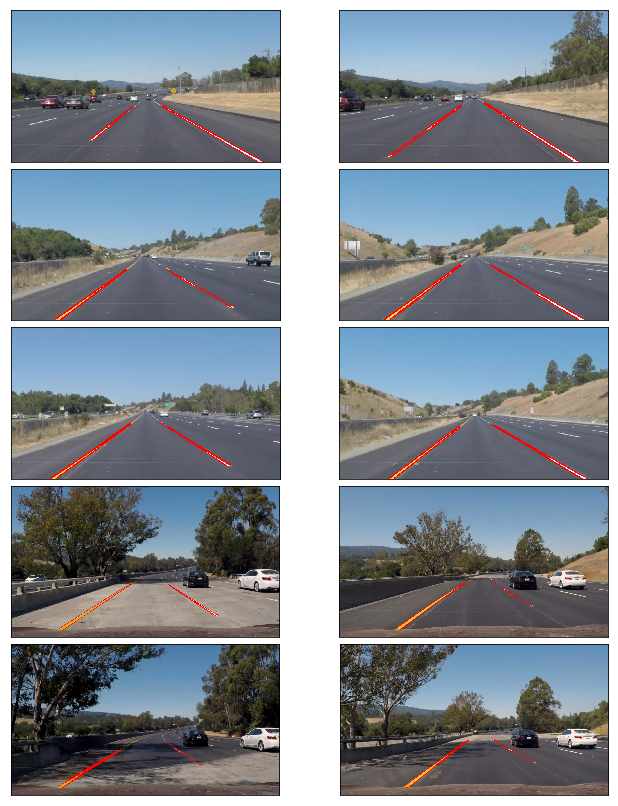
\includegraphics{test_images_output/hough_test_images.png}
\caption{Hough test images}
\end{figure}

\hypertarget{so-were-done-right-well-not-quite.}{%
\subsubsection{So we're done, right? well not
quite.}\label{so-were-done-right-well-not-quite.}}

The lane lines are clearly identified and a red line is drawn over the
line segments connecting most dashed lines segments; however, we can
still see the gaps in some of images where the lines are not connected
to the full extent of the lane lines.

\hypertarget{extrapolating-lane-lines}{%
\subsection{\#\# Extrapolating Lane
Lines}\label{extrapolating-lane-lines}}

I altered the \texttt{hough\_lines} to return a list of lines along with
the image with lines drawn on them, I did this because these lines will
be divided into right and left lane lines, averaged, and weighted to
produce the best fit for the lane lines.

After finding the lane lines and drawing them I extrapolated (extended)
the lane lines to have two continues lane lines from the bottom of the
image (the car's body) and towards the horizon (60\% of the image). I
achieve this by:

\begin{itemize}
\tightlist
\item
  Section \ref{averaging20lanelines}
\item
  Section \ref{making20lines20to20draw}
\item
  Section \ref{drawing20the20lane20lines}
\end{itemize}

\hypertarget{averaging-lanelines}{%
\paragraph{Averaging LaneLines}\label{averaging-lanelines}}

I wrote a method \texttt{average\_slope\_yintercept} that returns two
lane lines (slope, y-intercept) by dividing our lane lines as left and
right using their slopes \emph{negative} slope means \emph{left lane}
and \emph{positive} means \emph{right lane} (inversed), then I averaged
each lane line \emph{slopes} and \emph{y-intercepts} to get a single
line for each lane. Also I used each \emph{line length} as a
\emph{weight} to give more consideration to lines that are \emph{longer}
in length.

\hypertarget{making-line-to-draw}{%
\paragraph{Making Line to Draw}\label{making-line-to-draw}}

Then I made lines for the averaged lane lines from their \textbf{slopes}
and \textbf{y-intercepts} using the straight line equation
\texttt{y\ =\ mx\ +\ b}

\hypertarget{drawing-the-lane-lines}{%
\paragraph{Drawing the Lane Lines}\label{drawing-the-lane-lines}}

I decided to make \texttt{draw\_lane\_lines()} method to handle drawing
the extrapolated lane lines instead of altering \texttt{draw\_lines()}
method for better code organization, so basically
\texttt{draw\_lane\_lines()} is my modified \texttt{draw\_lines()}.

Here are the results of the \texttt{draw\_lane\_lines()}
``darw\_line()'' method:
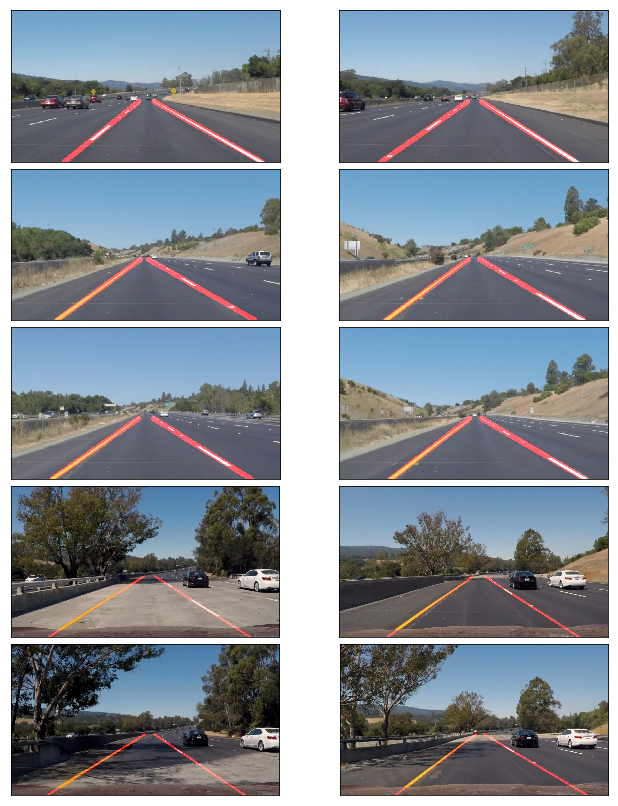
\includegraphics{test_images_output/extrapolated_test_images.png}

\hypertarget{one-more-thing-averaging-video-frames}{%
\subsection{\#\# One more thing (Averaging video
frames)}\label{one-more-thing-averaging-video-frames}}

\hypertarget{done}{%
\subsubsection{Done?}\label{done}}

Actually still one more thing. After applying the pipeline on the first
video \textbf{solidWhiteRight} the result seemed ok though the lines
were a little jittery. However, when applying it to the second video
\textbf{solidYellowLeft} i noticed that at a certain second in the video
the lane lines crossed each other for as you can see here:
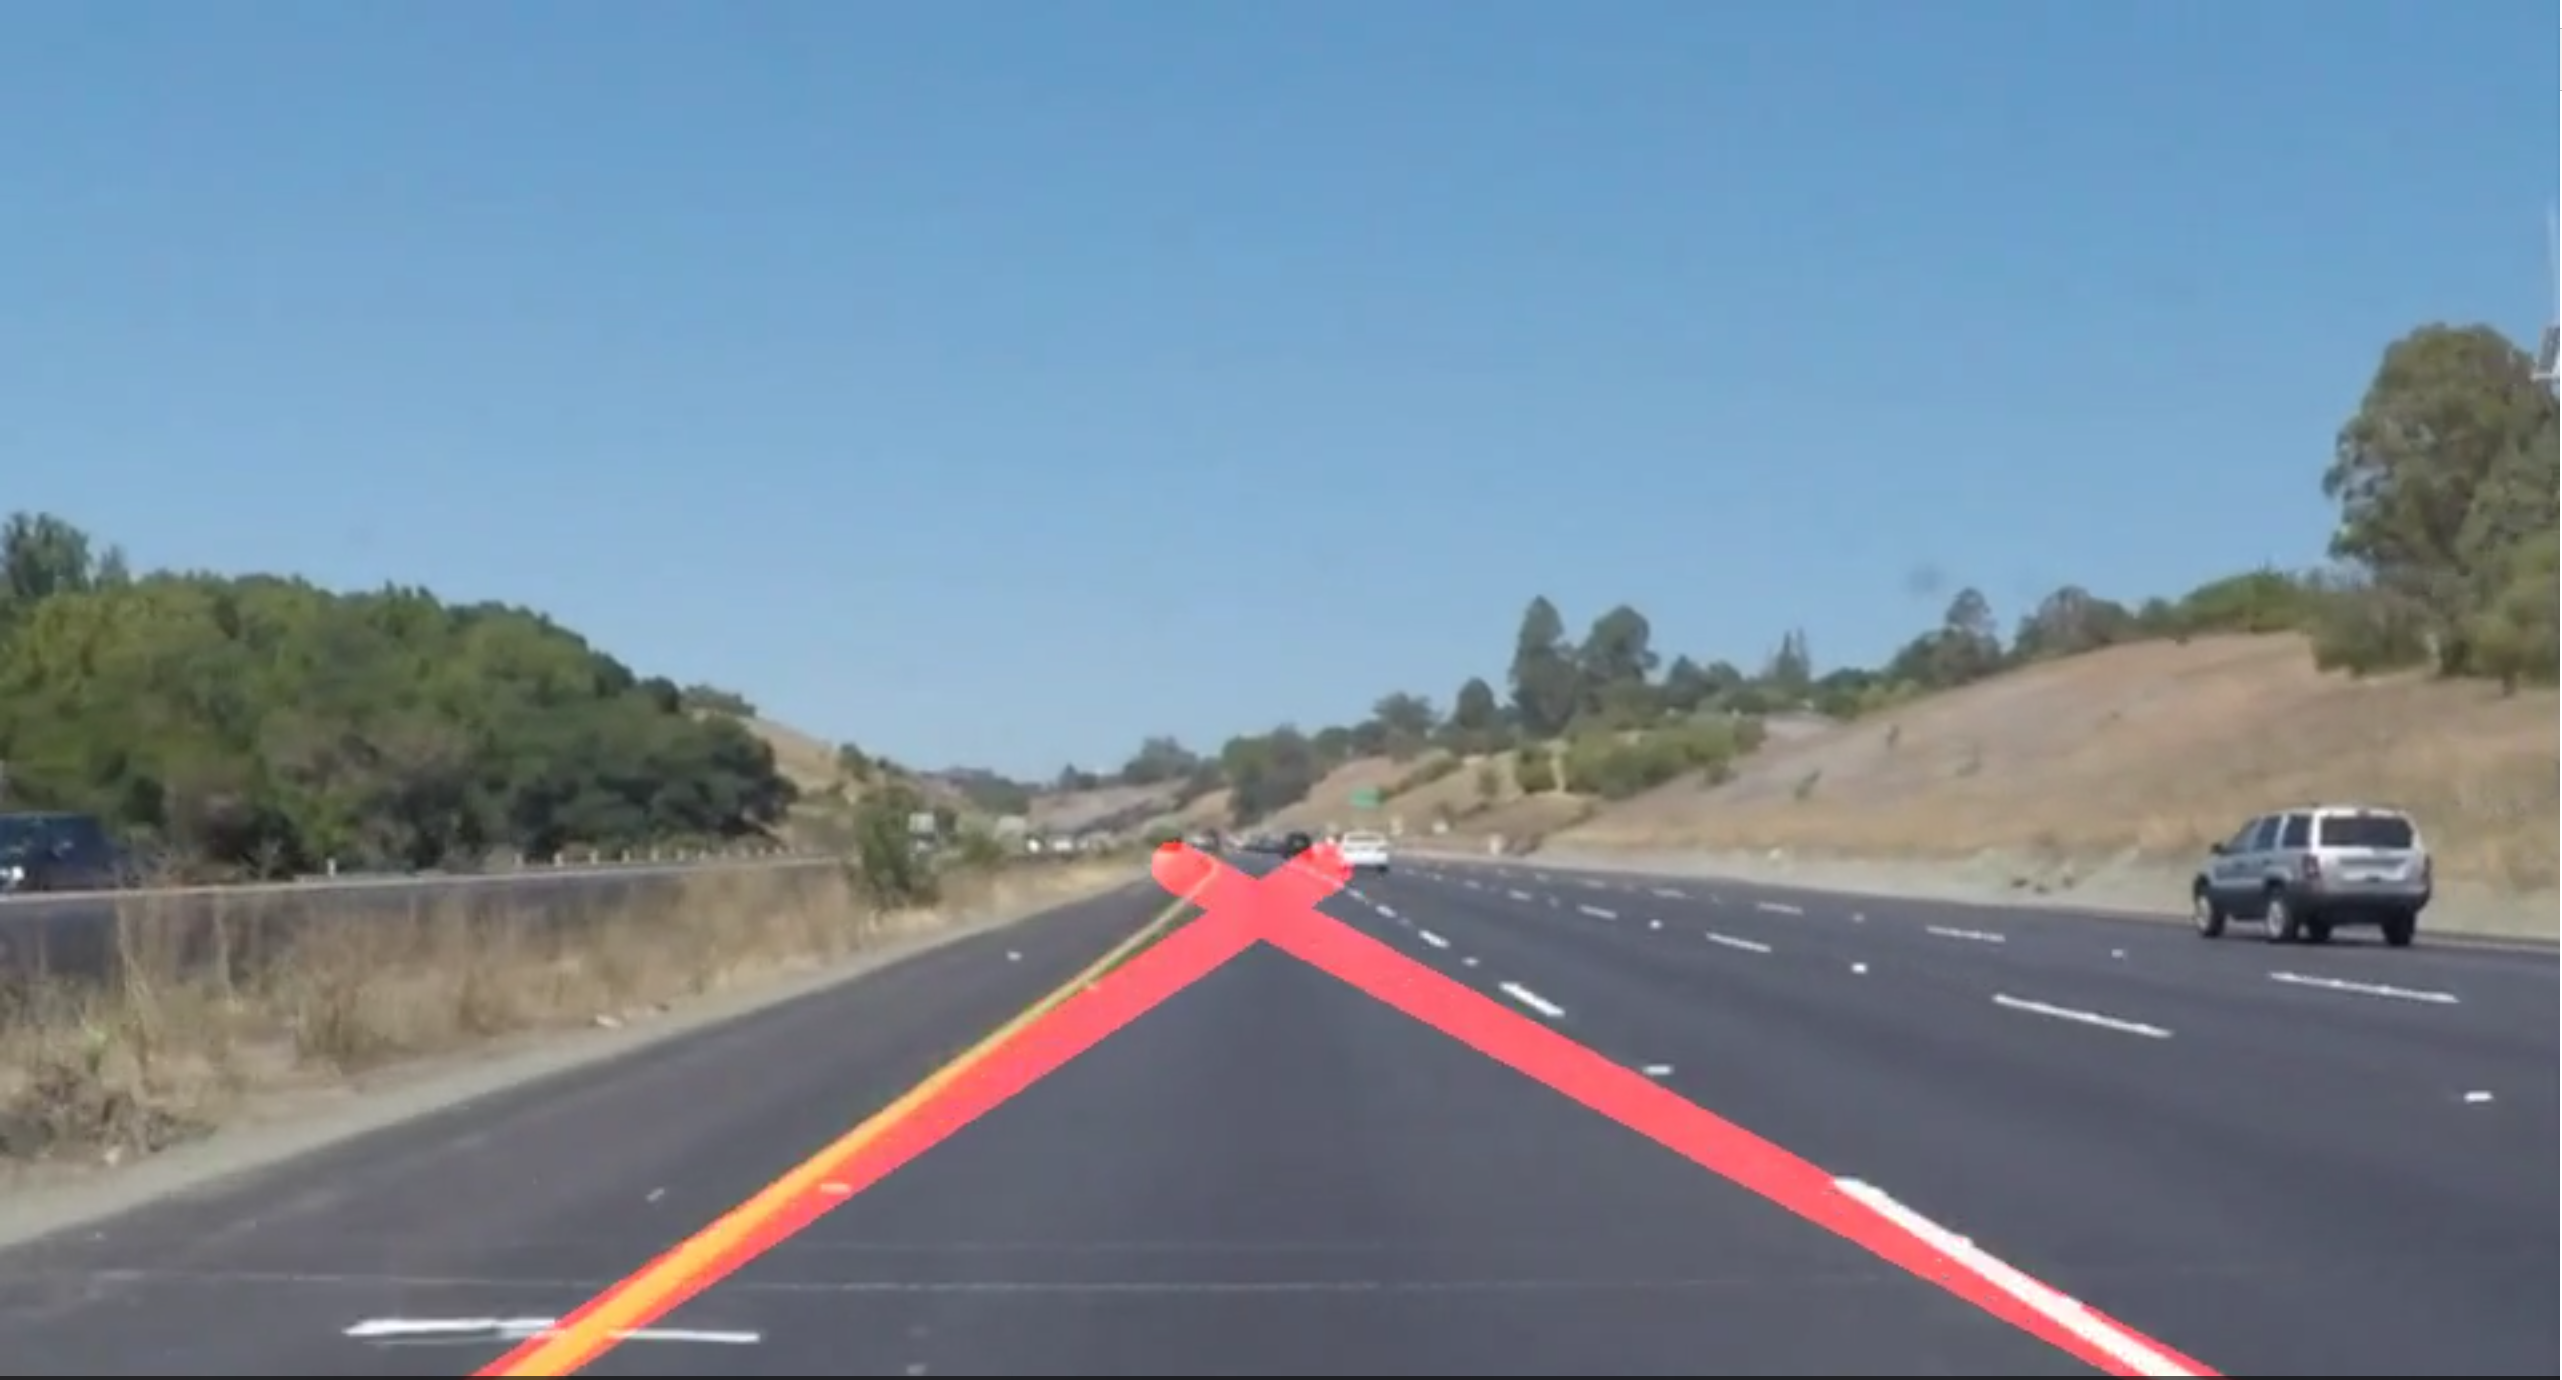
\includegraphics{test_images_output/crossed_lines.png}

Since videos mainly play 60 frames per second and each frame is an
image, therefore I averaged the frames' lines to have a smoother and
more consistent lane lines that didn't jitter and cross each other due
to a couple of faulty frames. I chose to average across a \textbf{30}
frame sample, this number gave me the most stable results.

So I made a \texttt{class} called \texttt{LaneLineFinder} with: *
\texttt{SAMPLE\_FRAMES} as a \emph{constant} number of frames to average
across * \texttt{right\_lane\_lines} and \texttt{left\_lane\_lines} are
two \texttt{deque} (queue in python) variables of length
\texttt{SAMPLE\_FRAMES}\\
* \texttt{average\_line\_sampling} gets the average of the previous
\texttt{SAMPLE\_FRAMES} frames using numpy \texttt{np.mean} method *
\texttt{process\_image} which executes the pipeline

\hypertarget{video-links}{%
\subsection{\#\# Video links}\label{video-links}}

You can checkout the full video processed videos in the links provided
below:

\begin{itemize}
\tightlist
\item
  \href{https://youtu.be/kV6LGD-cY3I}{Solid white right}
\item
  \href{https://youtu.be/iUBEwLEFOYI}{Solid yellow left}
\item
  \href{https://youtu.be/MwuveIP4Lpc}{Challenge}
\end{itemize}

    \hypertarget{potential-shortcomings-with-the-pipeline}{%
\subsection{2. Potential shortcomings with the
pipeline}\label{potential-shortcomings-with-the-pipeline}}

Here are so shortcoming that I need to address in the coming weeks as I
advance through the course:

\begin{enumerate}
\def\labelenumi{\arabic{enumi}.}
\tightlist
\item
  Identifying curves and curving my extrapolated lines accordingly.
\item
  It also seems that the line quality is tested when the car is driving
  at higher speeds.
\item
  I need a more robust and dynamic way of identifying the road's horizon
  rather than just including 60\% of the image hight.
\item
  I don't know what will be the case if there is a car close and in the
  same lane us our line of site, also what will be the case if the car
  is either white or yellow?
\item
  Will this algorithm work in low light situation?
\end{enumerate}

    \hypertarget{possible-improvements-could-be}{%
\subsection{3. Possible improvements could
be}\label{possible-improvements-could-be}}

\begin{enumerate}
\def\labelenumi{\arabic{enumi}.}
\tightlist
\item
  Identifying the horizon using a color filter as I did with the lane
  lines using the tarmac, or asphalt color.
\item
  Ignoring horizontal lines to make the pipeline immune to close cars in
  the same lane.
\item
  Using a different detection method that deals with higher order
  polynomial to account for curved lines
\end{enumerate}


    % Add a bibliography block to the postdoc
    
    
    
    \end{document}
